% --
% game kws integration

\section{Keyword Spotting System Integration}
The use of KWS in a video game requires the integration of a dedicated system within the game framework.
The KWS system deployed in this thesis consists of two essential parts: An online system and a classification system.
The online system captures the audio stream input from a microphone in real-time and stores it in a FIFO (First In First Out) queue for subsequent calculations of features and keyword prediction in the classification system.
The classification system consists of a feature extractor and the neural network architecture for the KWS task.
The video game interprets the commands from the classification systems and performs the resulting actions within the game.
More detailed descriptions of the individual sub systems are provided below.


% --
% online

\subsection{Online System}
The online system is mainly composed of a FIFO queue for input data storage and an energy onset detection method.
The length of the FIFO queue has to be at least as large as the sample length of the speech command examples used to train the neural networks for classification.
The recorded files in the speech command dataset have a time duration of \SI{1}{\second}. 
Using this time duration however would have made the classification of keywords very slow and influenced the gaming experience.
In this thesis, the length of a keyword is restricted to \SI{500}{\milli\second} or 8000 samples.
Furthermore, some buffer samples are added for an improved detection of the highest energy region within the speech signal.
Note that the input stream reads out the microphone data in chunks, where the length of each chunk had been chosen to be 160 samples, corresponding to exactly one frame with hop size of \SI{10}{\milli\second}.
Ideally these buffer frames should not be necessary but due to shift invariance problems in some network architectures (especially for the \texttt{fstride} model) it can be advantageous and improve the keyword predictions when buffer frames are added.

The buffer frames are located prior and posterior to the dedicated keyword frames and were both selected to have a length of 5 frames.
Essentially, the buffer frames extend the keyword frames but can also be seen as queues by themselves.
Therefore, the whole FIFO queue consist of three individual queues: the prior buffer queue, the key word queue, and the posterior buffer queue.
The prior buffer queue consecutively collects the frames from the audio stream but does not feed the output to the key word queue as long as there is no keyword onset detected.
Each input chunk or frame is used for the detection of an online onset, as described in \rsec{signal_onset_online}.
If an onset is detected from one of these frames, subsequently the whole FIFO queue will be filled up to its full size including the posterior buffer frames.
Afterwards the frames contained in the FIFO queue are read out and passed to the feature extraction module, which is already located in the classification system.
The scheme of the online system with integrated FIFO queue is illustrated in \rfig{game_system_online}.
\begin{figure}[!ht]
  \centering
  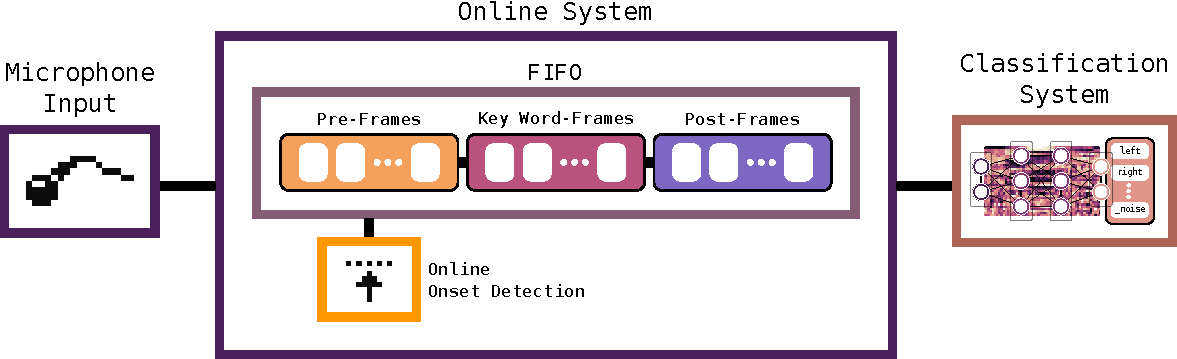
\includegraphics[width=0.9\textwidth]{./6_game/figs/game_system_online.pdf}
  \caption{Scheme of the online system with FIFO structure.}
  \label{fig:game_system_online}
\end{figure}
\FloatBarrier
\noindent


% --
% classification

\subsection{Classification System}
The classification system consists of a feature extractor and a classifier, which further composes of a neural network architecture for the classification of the keywords it was trained for.
The feature extractor computes the MFCCs according to its provided feature extraction parameters and determines the highest energy onset as described in \rsec{signal_onset_kw}.
The feature extraction parameters provide information about the exact constellation of features used during training, for instance 12 MFCC coefficients with frame-based normalization and no feature enhancements.
This ensures the application of the same feature extraction to new data frames from the online system.

The classifier requires the unique name of the trained neural network model, such as \texttt{conv-jim}, the parameters of this model, and the class dictionary.
The trained weights of the  models are stored in the \texttt{.pth} format used within the \texttt{Pytorch} framework and can simply be loaded to a corresponding model architecture.
The class dictionary describes which output node of the neural network corresponds to which speech command and is especially important for the video game to trigger correct actions.
After loading the parameters the classifier simply performs an inference to the most probable keyword in its class dictionary.

A game action is elicited once a keyword is present from the classification system.
This can, for example, be implemented by using an input handler similar to a keyboard input handler or event system that is listening for new speech commands and triggers an action when one is available.
\rfig{game_system_classification} shows a scheme of the classification system.
\begin{figure}[!ht]
  \centering
  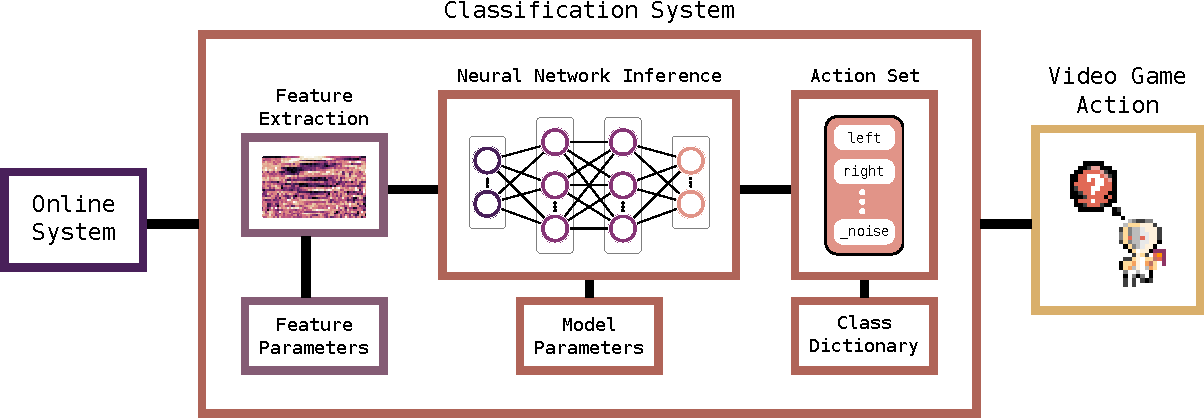
\includegraphics[width=0.9\textwidth]{./6_game/figs/game_system_classification.pdf}
  \caption{Scheme of the classification system.}
  \label{fig:game_system_classification}
\end{figure}
\FloatBarrier
\noindent

